%--------------
%% preamble.tex
%% this should be included with a command like
%% %--------------
%% preamble.tex
%% this should be included with a command like
%% %--------------
%% preamble.tex
%% this should be included with a command like
%% \input{preamble.tex}
%% Template based on Aleksander Madry's and Dan Spielman's template
\documentclass[12pt]{article}
%\renewcommand{\baselinestretch}{1.5}
\usepackage[OT4]{fontenc}
\newtheorem{define}{Definition}
\usepackage{amsmath}
\usepackage{graphicx}
\usepackage{enumitem}
\usepackage{float}
\usepackage{color}

\oddsidemargin=0.15in
\evensidemargin=0.15in
\topmargin=-.5in
\textheight=9in
\textwidth=6.25in

\renewcommand{\thefootnote}{\fnsymbol{footnote}}

\hbadness=10000
\vbadness=10000

%\setlength{\oddsidemargin}{.1in}
%\setlength{\evensidemargin}{.1in}
%\setlength{\textwidth}{6in}
\setlength{\topmargin}{-0.4in}
\setlength{\textheight}{8.5in}

\newcommand{\handout}[5]{
	\noindent
	\begin{center}
		\framebox{
			\vbox{
				\hbox to 5.78in { {\bf #1}
					\hfill #2 }
				\vspace{4mm}
				\hbox to 5.78in { {\Large \hfill #5  \hfill} }
				\vspace{2mm}
				\hbox to 5.78in { {\it #3 \hfill #4} }
			}
		}
	\end{center}
	\vspace*{4mm}
}

\newcommand{\header}[3]{\handout{NUS CS-CS5562: Trustworthy Machine Learning}{\today}{Lecturer: Reza Shokri}{Student: #2\quad#3}{#1}}


\newtheorem{theorem}{Theorem}
\newtheorem{corollary}[theorem]{Corollary}
\newtheorem{lemma}[theorem]{Lemma}
\newtheorem{observation}[theorem]{Observation}
\newtheorem{proposition}[theorem]{Proposition}
\newtheorem{definition}[theorem]{Definition}
\newtheorem{claim}[theorem]{Claim}
\newtheorem{fact}[theorem]{Fact}
\newtheorem{assumption}[theorem]{Assumption}

\newcommand{\qed}{\rule{7pt}{7pt}}
\newcommand{\dis}{\mathop{\mbox{\rm d}}\nolimits}
\newcommand{\per}{\mathop{\mbox{\rm per}}\nolimits}
\newcommand{\area}{\mathop{\mbox{\rm area}}\nolimits}
\newcommand{\cw}{\mathop{\rm cw}\nolimits}
\newcommand{\ccw}{\mathop{\rm ccw}\nolimits}
\newcommand{\DIST}{\mathop{\mbox{\rm DIST}}\nolimits}
\newcommand{\OP}{\mathop{\mbox{\it OP}}\nolimits}
\newcommand{\OPprime}{\mathop{\mbox{\it OP}^{\,\prime}}\nolimits}
\newcommand{\ihat}{\hat{\imath}}
\newcommand{\jhat}{\hat{\jmath}}
\newcommand{\abs}[1]{\mathify{\left| #1 \right|}}

\newenvironment{proof}{\noindent{\bf Proof}\hspace*{1em}}{\qed\bigskip}
\newenvironment{proof-sketch}{\noindent{\bf Sketch of Proof}\hspace*{1em}}{\qed\bigskip}
\newenvironment{proof-idea}{\noindent{\bf Proof Idea}\hspace*{1em}}{\qed\bigskip}
\newenvironment{proof-of-lemma}[1]{\noindent{\bf Proof of Lemma #1}\hspace*{1em}}{\qed\bigskip}
\newenvironment{proof-attempt}{\noindent{\bf Proof Attempt}\hspace*{1em}}{\qed\bigskip}
\newenvironment{proofof}[1]{\noindent{\bf Proof}
of #1:\hspace*{1em}}{\qed\bigskip}
\newenvironment{remark}{\noindent{\bf Remark}\hspace*{1em}}{\bigskip}

% \makeatletter
% \@addtoreset{figure}{section}
% \@addtoreset{table}{section}
% \@addtoreset{equation}{section}
% \makeatother

\newcommand{\FOR}{{\bf for}}
\newcommand{\TO}{{\bf to}}
\newcommand{\DO}{{\bf do}}
\newcommand{\WHILE}{{\bf while}}
\newcommand{\AND}{{\bf and}}
\newcommand{\IF}{{\bf if}}
\newcommand{\THEN}{{\bf then}}
\newcommand{\ELSE}{{\bf else}}

% \renewcommand{\thefigure}{\thesection.\arabic{figure}}
% \renewcommand{\thetable}{\thesection.\arabic{table}}
% \renewcommand{\theequation}{\thesection.\arabic{equation}}

\makeatletter
\def\fnum@figure{{\bf Figure \thefigure}}
\def\fnum@table{{\bf Table \thetable}}
\long\def\@mycaption#1[#2]#3{\addcontentsline{\csname
  ext@#1\endcsname}{#1}{\protect\numberline{\csname
  the#1\endcsname}{\ignorespaces #2}}\par
  \begingroup
    \@parboxrestore
    \small
    \@makecaption{\csname fnum@#1\endcsname}{\ignorespaces #3}\par
  \endgroup}
\def\mycaption{\refstepcounter\@captype \@dblarg{\@mycaption\@captype}}
\makeatother

\newcommand{\figcaption}[1]{\mycaption[]{#1}}
\newcommand{\tabcaption}[1]{\mycaption[]{#1}}
\newcommand{\head}[1]{\chapter[Lecture \##1]{}}
\newcommand{\mathify}[1]{\ifmmode{#1}\else\mbox{$#1$}\fi}
%\renewcommand{\Pr}[1]{\mathify{\mbox{Pr}\left[#1\right]}}
%\newcommand{\Exp}[1]{\mathify{\mbox{Exp}\left[#1\right]}}
\newcommand{\bigO}O
\newcommand{\set}[1]{\mathify{\left\{ #1 \right\}}}
\def\half{\frac{1}{2}}

\newcommand{\fig}[4]{
        \begin{figure}
        \setlength{\epsfysize}{#2}
        \vspace{3mm}
        \centerline{\epsfbox{#4}}
        \caption{#3} \label{#1}
        \end{figure}
        }

\newcommand{\ord}{{\rm ord}}

\providecommand{\norm}[1]{\lVert #1 \rVert}
\newcommand{\embed}{{\rm Embed}}
\newcommand{\qembed}{\mbox{$q$-Embed}}
\newcommand{\calh}{{\cal H}}
\newcommand{\lp}{{\rm LP}}

\newcounter{mysolctr}

\newenvironment{mysolution}% environment name
{% begin code
	\refstepcounter{mysolctr}
	\color{blue}
	\par\vspace{\baselineskip}%
	\textbf{Solution \themysolctr}%
	\par\vspace{\baselineskip}%
}%
{}% end code
\numberwithin{mysolctr}{section}

\newenvironment{pts}% environment name
{% begin code
	\color{red}
	\par\vspace{\baselineskip}%
	\textbf{Points Scheme}%
	\par\vspace{\baselineskip}%
}%
{}% end code 

%% Template based on Aleksander Madry's and Dan Spielman's template
\documentclass[12pt]{article}
%\renewcommand{\baselinestretch}{1.5}
\usepackage[OT4]{fontenc}
\newtheorem{define}{Definition}
\usepackage{amsmath}
\usepackage{graphicx}
\usepackage{enumitem}
\usepackage{float}
\usepackage{color}

\oddsidemargin=0.15in
\evensidemargin=0.15in
\topmargin=-.5in
\textheight=9in
\textwidth=6.25in

\renewcommand{\thefootnote}{\fnsymbol{footnote}}

\hbadness=10000
\vbadness=10000

%\setlength{\oddsidemargin}{.1in}
%\setlength{\evensidemargin}{.1in}
%\setlength{\textwidth}{6in}
\setlength{\topmargin}{-0.4in}
\setlength{\textheight}{8.5in}

\newcommand{\handout}[5]{
	\noindent
	\begin{center}
		\framebox{
			\vbox{
				\hbox to 5.78in { {\bf #1}
					\hfill #2 }
				\vspace{4mm}
				\hbox to 5.78in { {\Large \hfill #5  \hfill} }
				\vspace{2mm}
				\hbox to 5.78in { {\it #3 \hfill #4} }
			}
		}
	\end{center}
	\vspace*{4mm}
}

\newcommand{\header}[3]{\handout{NUS CS-CS5562: Trustworthy Machine Learning}{\today}{Lecturer: Reza Shokri}{Student: #2\quad#3}{#1}}


\newtheorem{theorem}{Theorem}
\newtheorem{corollary}[theorem]{Corollary}
\newtheorem{lemma}[theorem]{Lemma}
\newtheorem{observation}[theorem]{Observation}
\newtheorem{proposition}[theorem]{Proposition}
\newtheorem{definition}[theorem]{Definition}
\newtheorem{claim}[theorem]{Claim}
\newtheorem{fact}[theorem]{Fact}
\newtheorem{assumption}[theorem]{Assumption}

\newcommand{\qed}{\rule{7pt}{7pt}}
\newcommand{\dis}{\mathop{\mbox{\rm d}}\nolimits}
\newcommand{\per}{\mathop{\mbox{\rm per}}\nolimits}
\newcommand{\area}{\mathop{\mbox{\rm area}}\nolimits}
\newcommand{\cw}{\mathop{\rm cw}\nolimits}
\newcommand{\ccw}{\mathop{\rm ccw}\nolimits}
\newcommand{\DIST}{\mathop{\mbox{\rm DIST}}\nolimits}
\newcommand{\OP}{\mathop{\mbox{\it OP}}\nolimits}
\newcommand{\OPprime}{\mathop{\mbox{\it OP}^{\,\prime}}\nolimits}
\newcommand{\ihat}{\hat{\imath}}
\newcommand{\jhat}{\hat{\jmath}}
\newcommand{\abs}[1]{\mathify{\left| #1 \right|}}

\newenvironment{proof}{\noindent{\bf Proof}\hspace*{1em}}{\qed\bigskip}
\newenvironment{proof-sketch}{\noindent{\bf Sketch of Proof}\hspace*{1em}}{\qed\bigskip}
\newenvironment{proof-idea}{\noindent{\bf Proof Idea}\hspace*{1em}}{\qed\bigskip}
\newenvironment{proof-of-lemma}[1]{\noindent{\bf Proof of Lemma #1}\hspace*{1em}}{\qed\bigskip}
\newenvironment{proof-attempt}{\noindent{\bf Proof Attempt}\hspace*{1em}}{\qed\bigskip}
\newenvironment{proofof}[1]{\noindent{\bf Proof}
of #1:\hspace*{1em}}{\qed\bigskip}
\newenvironment{remark}{\noindent{\bf Remark}\hspace*{1em}}{\bigskip}

% \makeatletter
% \@addtoreset{figure}{section}
% \@addtoreset{table}{section}
% \@addtoreset{equation}{section}
% \makeatother

\newcommand{\FOR}{{\bf for}}
\newcommand{\TO}{{\bf to}}
\newcommand{\DO}{{\bf do}}
\newcommand{\WHILE}{{\bf while}}
\newcommand{\AND}{{\bf and}}
\newcommand{\IF}{{\bf if}}
\newcommand{\THEN}{{\bf then}}
\newcommand{\ELSE}{{\bf else}}

% \renewcommand{\thefigure}{\thesection.\arabic{figure}}
% \renewcommand{\thetable}{\thesection.\arabic{table}}
% \renewcommand{\theequation}{\thesection.\arabic{equation}}

\makeatletter
\def\fnum@figure{{\bf Figure \thefigure}}
\def\fnum@table{{\bf Table \thetable}}
\long\def\@mycaption#1[#2]#3{\addcontentsline{\csname
  ext@#1\endcsname}{#1}{\protect\numberline{\csname
  the#1\endcsname}{\ignorespaces #2}}\par
  \begingroup
    \@parboxrestore
    \small
    \@makecaption{\csname fnum@#1\endcsname}{\ignorespaces #3}\par
  \endgroup}
\def\mycaption{\refstepcounter\@captype \@dblarg{\@mycaption\@captype}}
\makeatother

\newcommand{\figcaption}[1]{\mycaption[]{#1}}
\newcommand{\tabcaption}[1]{\mycaption[]{#1}}
\newcommand{\head}[1]{\chapter[Lecture \##1]{}}
\newcommand{\mathify}[1]{\ifmmode{#1}\else\mbox{$#1$}\fi}
%\renewcommand{\Pr}[1]{\mathify{\mbox{Pr}\left[#1\right]}}
%\newcommand{\Exp}[1]{\mathify{\mbox{Exp}\left[#1\right]}}
\newcommand{\bigO}O
\newcommand{\set}[1]{\mathify{\left\{ #1 \right\}}}
\def\half{\frac{1}{2}}

\newcommand{\fig}[4]{
        \begin{figure}
        \setlength{\epsfysize}{#2}
        \vspace{3mm}
        \centerline{\epsfbox{#4}}
        \caption{#3} \label{#1}
        \end{figure}
        }

\newcommand{\ord}{{\rm ord}}

\providecommand{\norm}[1]{\lVert #1 \rVert}
\newcommand{\embed}{{\rm Embed}}
\newcommand{\qembed}{\mbox{$q$-Embed}}
\newcommand{\calh}{{\cal H}}
\newcommand{\lp}{{\rm LP}}

\newcounter{mysolctr}

\newenvironment{mysolution}% environment name
{% begin code
	\refstepcounter{mysolctr}
	\color{blue}
	\par\vspace{\baselineskip}%
	\textbf{Solution \themysolctr}%
	\par\vspace{\baselineskip}%
}%
{}% end code
\numberwithin{mysolctr}{section}

\newenvironment{pts}% environment name
{% begin code
	\color{red}
	\par\vspace{\baselineskip}%
	\textbf{Points Scheme}%
	\par\vspace{\baselineskip}%
}%
{}% end code 

%% Template based on Aleksander Madry's and Dan Spielman's template
\documentclass[12pt]{article}
%\renewcommand{\baselinestretch}{1.5}
\usepackage[OT4]{fontenc}
\newtheorem{define}{Definition}
\usepackage{amsmath}
\usepackage{graphicx}
\usepackage{enumitem}
\usepackage{float}
\usepackage{color}

\oddsidemargin=0.15in
\evensidemargin=0.15in
\topmargin=-.5in
\textheight=9in
\textwidth=6.25in

\renewcommand{\thefootnote}{\fnsymbol{footnote}}

\hbadness=10000
\vbadness=10000

%\setlength{\oddsidemargin}{.1in}
%\setlength{\evensidemargin}{.1in}
%\setlength{\textwidth}{6in}
\setlength{\topmargin}{-0.4in}
\setlength{\textheight}{8.5in}

\newcommand{\handout}[5]{
	\noindent
	\begin{center}
		\framebox{
			\vbox{
				\hbox to 5.78in { {\bf #1}
					\hfill #2 }
				\vspace{4mm}
				\hbox to 5.78in { {\Large \hfill #5  \hfill} }
				\vspace{2mm}
				\hbox to 5.78in { {\it #3 \hfill #4} }
			}
		}
	\end{center}
	\vspace*{4mm}
}

\newcommand{\header}[3]{\handout{NUS CS-CS5562: Trustworthy Machine Learning}{\today}{Lecturer: Reza Shokri}{Student: #2\quad#3}{#1}}


\newtheorem{theorem}{Theorem}
\newtheorem{corollary}[theorem]{Corollary}
\newtheorem{lemma}[theorem]{Lemma}
\newtheorem{observation}[theorem]{Observation}
\newtheorem{proposition}[theorem]{Proposition}
\newtheorem{definition}[theorem]{Definition}
\newtheorem{claim}[theorem]{Claim}
\newtheorem{fact}[theorem]{Fact}
\newtheorem{assumption}[theorem]{Assumption}

\newcommand{\qed}{\rule{7pt}{7pt}}
\newcommand{\dis}{\mathop{\mbox{\rm d}}\nolimits}
\newcommand{\per}{\mathop{\mbox{\rm per}}\nolimits}
\newcommand{\area}{\mathop{\mbox{\rm area}}\nolimits}
\newcommand{\cw}{\mathop{\rm cw}\nolimits}
\newcommand{\ccw}{\mathop{\rm ccw}\nolimits}
\newcommand{\DIST}{\mathop{\mbox{\rm DIST}}\nolimits}
\newcommand{\OP}{\mathop{\mbox{\it OP}}\nolimits}
\newcommand{\OPprime}{\mathop{\mbox{\it OP}^{\,\prime}}\nolimits}
\newcommand{\ihat}{\hat{\imath}}
\newcommand{\jhat}{\hat{\jmath}}
\newcommand{\abs}[1]{\mathify{\left| #1 \right|}}

\newenvironment{proof}{\noindent{\bf Proof}\hspace*{1em}}{\qed\bigskip}
\newenvironment{proof-sketch}{\noindent{\bf Sketch of Proof}\hspace*{1em}}{\qed\bigskip}
\newenvironment{proof-idea}{\noindent{\bf Proof Idea}\hspace*{1em}}{\qed\bigskip}
\newenvironment{proof-of-lemma}[1]{\noindent{\bf Proof of Lemma #1}\hspace*{1em}}{\qed\bigskip}
\newenvironment{proof-attempt}{\noindent{\bf Proof Attempt}\hspace*{1em}}{\qed\bigskip}
\newenvironment{proofof}[1]{\noindent{\bf Proof}
of #1:\hspace*{1em}}{\qed\bigskip}
\newenvironment{remark}{\noindent{\bf Remark}\hspace*{1em}}{\bigskip}

% \makeatletter
% \@addtoreset{figure}{section}
% \@addtoreset{table}{section}
% \@addtoreset{equation}{section}
% \makeatother

\newcommand{\FOR}{{\bf for}}
\newcommand{\TO}{{\bf to}}
\newcommand{\DO}{{\bf do}}
\newcommand{\WHILE}{{\bf while}}
\newcommand{\AND}{{\bf and}}
\newcommand{\IF}{{\bf if}}
\newcommand{\THEN}{{\bf then}}
\newcommand{\ELSE}{{\bf else}}

% \renewcommand{\thefigure}{\thesection.\arabic{figure}}
% \renewcommand{\thetable}{\thesection.\arabic{table}}
% \renewcommand{\theequation}{\thesection.\arabic{equation}}

\makeatletter
\def\fnum@figure{{\bf Figure \thefigure}}
\def\fnum@table{{\bf Table \thetable}}
\long\def\@mycaption#1[#2]#3{\addcontentsline{\csname
  ext@#1\endcsname}{#1}{\protect\numberline{\csname
  the#1\endcsname}{\ignorespaces #2}}\par
  \begingroup
    \@parboxrestore
    \small
    \@makecaption{\csname fnum@#1\endcsname}{\ignorespaces #3}\par
  \endgroup}
\def\mycaption{\refstepcounter\@captype \@dblarg{\@mycaption\@captype}}
\makeatother

\newcommand{\figcaption}[1]{\mycaption[]{#1}}
\newcommand{\tabcaption}[1]{\mycaption[]{#1}}
\newcommand{\head}[1]{\chapter[Lecture \##1]{}}
\newcommand{\mathify}[1]{\ifmmode{#1}\else\mbox{$#1$}\fi}
%\renewcommand{\Pr}[1]{\mathify{\mbox{Pr}\left[#1\right]}}
%\newcommand{\Exp}[1]{\mathify{\mbox{Exp}\left[#1\right]}}
\newcommand{\bigO}O
\newcommand{\set}[1]{\mathify{\left\{ #1 \right\}}}
\def\half{\frac{1}{2}}

\newcommand{\fig}[4]{
        \begin{figure}
        \setlength{\epsfysize}{#2}
        \vspace{3mm}
        \centerline{\epsfbox{#4}}
        \caption{#3} \label{#1}
        \end{figure}
        }

\newcommand{\ord}{{\rm ord}}

\providecommand{\norm}[1]{\lVert #1 \rVert}
\newcommand{\embed}{{\rm Embed}}
\newcommand{\qembed}{\mbox{$q$-Embed}}
\newcommand{\calh}{{\cal H}}
\newcommand{\lp}{{\rm LP}}

\newcounter{mysolctr}

\newenvironment{mysolution}% environment name
{% begin code
	\refstepcounter{mysolctr}
	\color{blue}
	\par\vspace{\baselineskip}%
	\textbf{Solution \themysolctr}%
	\par\vspace{\baselineskip}%
}%
{}% end code
\numberwithin{mysolctr}{section}

\newenvironment{pts}% environment name
{% begin code
	\color{red}
	\par\vspace{\baselineskip}%
	\textbf{Points Scheme}%
	\par\vspace{\baselineskip}%
}%
{}% end code 

\usepackage{hyperref}
\usepackage{booktabs}
\usepackage{comment}
\usepackage{natbib}
\usepackage{bbm}
\usepackage{mathtools}
\usepackage{amsfonts}
\usepackage{appendix}
\usepackage{csquotes}
\usepackage{amssymb}
\usepackage{listings}
\usepackage{float}
\usepackage{caption}
\usepackage{subcaption}
\lstset{
    frame = single,
    breaklines=true,
    basicstyle=\ttfamily}
\usepackage{tikz, forest}
\usepackage{natbib}

\DeclareMathOperator*{\maximize}{maximize}
\DeclareMathOperator*{\minimize}{minimize}


\begin{document}

% Indicate your name and your student number (e.g., A01xxx)
\header{Assignment 3}{Niharika Shrivastava}{A0254355A}

\section{Warm-up}
\subsection*{1.3 The Naive Membership Inference Attack}
\begin{enumerate}
    \item TP: 1484, TN: 1144, FP: 856, FN: 516
    \item Attack accuracy of the naive membership inference attack: 65.7\%
\end{enumerate}


\section{Membership Inference Attacks Using Loss Values}
\subsection*{2.1 $M_{loss}$ - Using Loss Values to Estimate a Single Threshold}

\subsubsection{Initial Metrics}
$T_{loss}$: 2.1, $Accuracy_{initial}$: 62.8\%

\subsubsection{Optimized Metrics}
$T_{loss}$: 1.0, $Accuracy_{max}$: 66.7\% \\

I set $T_{loss}$ to range from $[0.1 - 3]$ by looking at the histogram for the train and test dataset loss values. Following this, I generate the membership labels and the corresponding attack accuracy for each $T_{loss}$ and select the $T_{loss}$ value which gives maximum attack accuracy.

\begin{figure}[h]
    \centering
    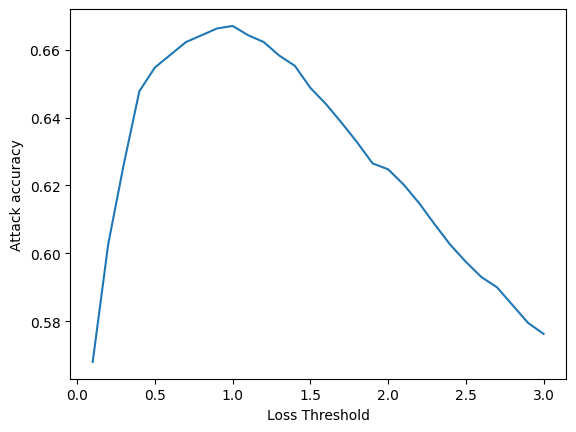
\includegraphics[width=0.47\textwidth]{quest2-1.png}
\end{figure}

\subsection*{2.2 $M_{loss, per\ class}$ - Using Loss Values to Estimate a Threshold for Each Class}
The classes that show the clearest distinction in the loss values are Class 2 and 3 (Fig. \ref{fig:quest2.2}).

\begin{figure}[h]
     \centering
     \begin{subfigure}[b]{0.49\textwidth}
         \centering
         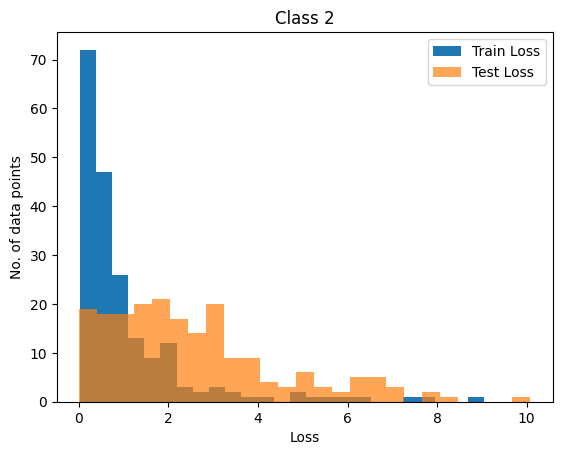
\includegraphics[width=\textwidth]{quest2-2.png}
     \end{subfigure}
     % \hfill
     \begin{subfigure}[b]{0.49\textwidth}
         \centering
         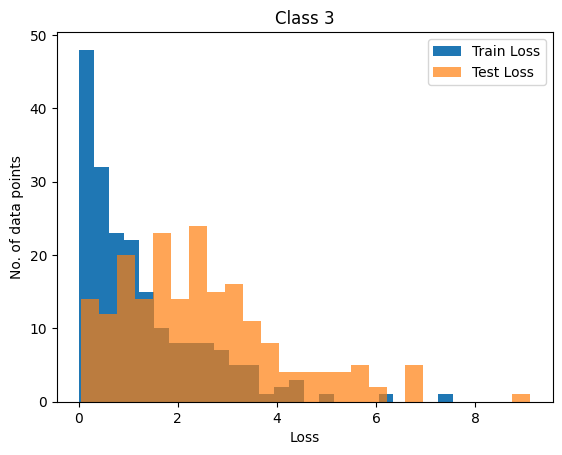
\includegraphics[width=\textwidth]{quest2-3.png}
     \end{subfigure}
        \caption{Distinction between losses}
        \label{fig:quest2.2}
\end{figure}

\subsubsection{Initial Metrics}
\begin{enumerate}
    \item $T_{loss, class i}$ = \{1, 1, 1, 1, 1, 1, 1, 1, 1, 1\}
    \item Attack accuracy for each class = $\{60, 61.5, 64, 58.4, 60.5, 64.4, 64.75, 65.2, 63, 64\}$
    \item Overall attack accuracy = 66.7\%
\end{enumerate}

\subsubsection{Optimized Metrics}
\begin{enumerate}
    \item $T_{loss, class i}$ = $\{0.4, 1.1, 1.0, 1.5, 0.6, 0.8, 0.4, 0.5, 0.8, 0.2\}$
    \item \% Attack accuracy for each class = $\{64, 70, 74.5, 69.5, 70.5, 67, 64.75, 67.75, 71, 66\}$
    \item Overall attack accuracy = 68.5\%
\end{enumerate}

To maximize the overall accuracy, I find the best $T_{loss, class i}$ for each class using the method described in section 2.0.2, i.e., find the $T_{loss, class i}$ for each class that maximizes the accuracy of that class. 

Compared with previous attacks, the attack accuracy is highest for $M_{loss, per class}$. This is because we are considering a new
piece of information that is the true class label of the input. We can see from the histograms that the distribution changes significantly depending on what class we are observing. If the distribution had been constant across all the classes
then $M_{loss, per class}$ accuracy would have been almost equal to $M_{loss}$.

\subsection*{2.3 Attacking a Model Trained With Regularization}
Attack accuracy for $M_{loss}$: 57.35\% \\
Attack accuracy for $M_{loss, per class}$: 59.68\% \\

Regularization generalizes the model performance on unseen data and not overfit on the training dataset. Therefore, the loss values on the train and test data are going to be very similar in case the model is regularized properly. In this case, choosing a $T_{loss}$ naively will not work well, as the number of false positives will increase, thereby bringing down the accuracy of the attack significantly. 

\section{Attacking the MLaaS Setting}
\begin{enumerate}
    \item Randomly sample n images from $D_{other,challenge}$ for each class.
    \item Split the above samples into n/2 train images and n/2 test images.
    \item Train k shadow models using the above-mentioned split.
    \item For each of the shadow model get the logits of their respective train and test dataset.
    \item Append the true class labels to the logits array and assign label 1 (MEMBER) for train dataset and 0 (NON-MEMBER) for test dataset records.
    \item Combine the above-mentioned datasets into $D_{train, attack}$. This will be used to train our attack model.
    \item The Attack model’s input is the logits along with the true class label. This is done because the prediction vector heavily depends on the true class label. Based on this, the attack model will classify it as 'MEMBER' or 'NON-MEMBER'.
    \item Attack model is a neural network with a single dense layer of 64 units.
    \item Once the attack model is trained, we pass the logits of $D_{eval,challenge}$ to generate the membership labels.
\end{enumerate}

\section{Testing Unintended Memorization}
    
\subsection*{4.1 Assessing a CNN Classifier on CIFAR10}

I set a threshold of 0.5 on memorization such that if the value is greater than 0.5, we can say with certainty that the model is memorizing. Otherwise, we cannot really comment on the model's memorizing power.

Based on this I selected 50 random data points and found out that for 17 data points
the model is memorizing with an average memorization value of 0.761. For all of these points,
the predicted labels of $h_{\theta}$ and $h`_{\theta}$ do not match. Therefore, we can say that the model is memorizing to a large extent.

\subsection*{4.2 Assessing an LSTM Next Character Predictor on Shakespeare Dataset}

Canary is: ”The random sequence is XXXX”. In the table below, we can see that there
is a correlation between number of repetitions and the relative perplexity. As the number
of repetitions k increase, the memorization also increases.

\begin{table}[h]
    \centering
    \begin{tabular}{cccccc}
        k & 2 & 5 & 10 & 20 & 50 \\
        Perplexity & 0.04261 & 1.583 &  3.3757 &  6.379 &  9.692 \\
    \end{tabular}
    \caption{Canary 1: ABCD}

    \vspace{0.5cm}

    \begin{tabular}{cccccc}
        k & 2 & 5 & 10 & 20 & 50 \\
        Perplexity & 3.08 &  3.17 & 4.65 & 5.44 & 22.75 \\
    \end{tabular}
    \caption{Canary 2: AHJB}
\end{table}

% \section{Training Data Reconstruction}

\end{document}
